\documentclass[letterpaper, 12pt]{article}
\usepackage{longtable, tabu, amsmath, amssymb, mathrsfs, graphicx, natbib}
\setlength{\parskip}{.5cm plus4mm minus3mm}

\begin{document}

\title{Indices for dynamic pricing in the event ticketing industry}
\author{\emph{Rohit Patel}\thanks{Kellogg School of Management}}
\date {March 25, 2018}
\maketitle
\begin{abstract} As dynamic pricing becomes more common for event tickets including NFL, MLB, NBA and NCAA games, the ability to effectively measure and track prices changes for an event over time becomes critical. Standard price measures that are currently used for price measurement are ill suited to capture the complexities of an event ticket. This article outlines new industry-specific measures for event tickets that enable lifecycle trend analysis for ticket prices and effective price tracking over time, adjusting for ticket quality and varying inventory. The measures introduced are designed to be invariant under large ticket sales, volume changes, and differences in seat values. Additionally, we also briefly discuss the impact of brokers on secondary market pricing to add to literature dynamics that remain presently unexplored
\end{abstract}
\noindent {\bf JEL Codes:} Z29, Z23, Z20, L83, L11, D49 \\
\noindent {\bf Keywords:} dynamic pricing, sports economics, event ticketing, sports analytics, ticket pricing

\section{Introduction}
The adoption of dynamic pricing has accelerated across all the major sports leagues in the past few years. However, there is limited empirical evidence that this has yielded increased revenues or other benefits.  In-fact, \cite{xu2017designing} investigate the matter for an MLB franchise and find that the return from dynamic pricing was $0.5\%$ lower than that from using a static pricing mechanism. This is despite the fact that dynamic pricing has been successfully deployed by multiple other industries. Moreover, \cite{xu2017designing} also estimate that with sufficient pricing flexibility, the franchise can achieve a potential revenue improvement of $17.2\%$ through dynamic pricing. This suggests a lack of proper execution of dynamic pricing in the event tickets sale industry. Much of the analysis is currently done using average ticket prices or standard pricing measures that are often ill suited to capture the complexities of an event ticket. Even for a particular event at a particular time, no two tickets are identical, and better analyzing ticket prices requires more specific measures suitable for the analysis. We provide tools to enable two types of analysis for purposes of improved dynamic pricing, and briefly discuss the impact of brokers on secondary market pricing - something that has been lacking in the current literature.

First, we define measures that will enable the analysis of an event to understand at what point of time in the lifecycle of the tickets sales is the volume concentrated. There is ample evidence (\cite{drayer2009value}, \cite{shapiro2012new}, \cite{kemper2015factors}) that ticket availability and prices depend on the number of days from the game. Yet there has been no research on how various events differ in their ability to attracts fans earlier or later in the ticket sales lifecycle. By providing measures that enable an empirical analysis of the events lifecycle, we hope to catalyze further research in this area and enhance understanding of the factors that can be key to successful dynamic pricing implementation.

Second, we propose pricing measures that enable tracking of price evolution over a period of time for an event. This is a key challenge when designing dynamic pricing systems since the inventory of tickets available for sale constantly changes from one day to another. This creates a challenge in fully understanding the reasons for price evolution due to the changing quality of seats. As an example, it is possible that prices were lower in period A than period B, and a higher number of premium tickets were sold in period A vs period B, making the average price (or any other existing price measures calculated) of the period A ticket sales higher than period B. This can complicate the efforts to understand the factors affecting dynamic price, especially as the reasons for ticket sales and the prices paid are likely to be correlated. \cite{paul2013determinants} make an effort to determine factors affecting dynamic price, however they use average prices which are likely to suffer from the aforementioned issue. We propose pricing measures that enables comparison of prices over time by adjusting for the changing inventory and the ticket quality available, thus enabling future researchers to empirically tackle the issue more effectively.

Lastly, we note that there is limited literature dealing with the impact of brokers on ticket pricing, and provide a very brief discussion on the topic.

\section{Review of related literature}
Pricing strategies for event tickets have evolved considerably in the past two decades from a cost plus approach, to variable pricing, leading up to widespread adoption of dynamic pricing. \cite{reese2001exploratory} first addressed the process of price setting by looking at NFL price setting mechanisms. \cite{howard2004tactics} similarly prove a review of tactics used by sports organizations to set prices and increase ticket sales. \cite{krautmann2007can} and \cite{coates2007ticket} address the question of tickets being priced in the inelastic range of demand by considering the complementarities between tickets sold and concessions. 

Looking into the factors responsible for ticket price differences, \cite{rishe2003ticket} explore cross-sectional differences in ticket prices across teams and causes for the size and direction of seasonal price increases in the National Football League (NFL) based on data from 1996-2001. Taking the first step in the direction of dynamic pricing, \cite{drayer2009value} analyze the ticket sell prices in the secondary market and identify that higher prices were associated with the number of bids, number of transactions, teams' winning percentage, city demographics, face value, day of the game, round of the playoffs, and number of days before the game that the ticket was sold. \cite{shapiro2012new} further look into dynamic pricing and the price differences between fixed ticket prices, dynamic prices and secondary market prices. \cite{kemper2015factors} similarly study ticket prices in the secondary market for Bundesliga tickets in Germany. While there is limited empirical evidence studying the effects of dynamic pricing in the event ticketing industry, \cite{xu2017designing} take the first step in the direction by analyzing the performance of a dynamic pricing strategy. 

While much of the research is focused on external factors affecting ticket prices, \cite{drayer2011examination}, \cite{nalbantis2017fans} and \cite{popp2018factors} focus attention on the customer's value of tickets, their willingness to pay, and the underlying factors.  \cite{drayer2011examination} find that the perceived value of the ticket is tied to the face value, and whether the fan was buying or selling the ticket. \cite{nalbantis2017fans} find that fans' notion of competitiveness of the game is the critical factor in the willingness to pay. \cite{popp2018factors} take a slightly different approach and jointly try to identify event related factors, fan characteristics and individual factors that contribute to high willingness to pay. They find that age, income, prior attendance, timing of purchase, and seat location influence the secondary market ticket price.

The remainder of the paper is structured as follows: In section~\ref{lcm} we describe the measures that enable analysis of lifecycle trends for event tickets. This is followed by section~\ref{prm} where we introduce new pricing measures for improved analysis of dynamic pricing systems. Lastly, we discuss broker participation in secondary markets and their impact in section~\ref{cip}. We assume that the analysis of ticket prices for dynamic pricing purposes is done using secondary market prices, and we denote the intermediary platform in which the prices are listed as $\mathcal{I}_0$. 

\section{Lifecycle analysis measure}\label{lcm}
A critical aspect of an effective dynamic pricing engine is the ability of extract the time value of a good. This means a good understanding of the sales patterns for various events, and why they arise is important. While visualization techniques can aid in understanding the value and volume of ticket sales at various points of time in the lifecycle of the event, they do not lend well to statistical analysis. Analyzing the underlying factors behind why certain events see increased sales toward the beginning vs others can be critical to effectively pricing the tickets at various points of time for events in the future. We propose statistical measures to this effect that can help with quantification of the phenomenon.

\noindent Let

\noindent $t_p$ - Date when the primary sale market opens\\
$t_r$ - Date when the secondary sale market opens (if different from primary)\\
$t_f$ - Date of the event\\ 

We divide the time period into deciles and mark the date that stands in the middle of resale and event date, $t_m = \frac{t_r+t_f}{2}$. For each decile, let $C(d)$ denote the total number of ticket sales in the $dth$ decile and $V(d)$ the total number of revenue in that decile for that event. Define:

\begin{align*}
	c(d) &= \frac{C(d)}{\sum_{i=1}^{10}C(i)}&\text{The proportion of sale (\# tickets) in a decile}\\
	v(d) &= \frac{V(d)}{\sum_{i=1}^{10}V(i)}&\text{The proportion of sale (GTV) in a decile}
\end{align*}

\noindent For each event calculate:
\begin{align*}
	&&M_c(e) &= \frac{1}{4}\left[\left\{\sum_{i=1}^{10} \left| \max(|i-5|,|i-6|) \cdot c(i) \right|\right\} -1 \right]\\
	or&&M_c(e) &= \frac{1}{4}\left[\left\{\sum_{i=1}^{5} \left[ (6-i) \cdot c(i) \right] +\sum_{i=6}^{10} \left[ (i-5) \cdot c(i) \right]\right\} -1 \right]
\end{align*}
And, 
\begin{align*}
  M'_c(e) &= \frac{1}{2} + \frac{1}{10}\left[\sum_{i=1}^{5} \left[ (i-6) \cdot c(i) \right] +\sum_{i=6}^{10} \left[ (i-5) \cdot c(i) \right]\right]\\
\end{align*}

\subsection{Properties and discussion}
The two measures work together to enable us to understand the trend. $M_c(e)$ varies between zero and one, where a value of zero signifies that all the sales are concentrated in the $5^{th}$ and the $6^{th}$ deciles, rather than earlier or later in the lifecycle. A value of one signifies the sales were concentrated entirely in the first or the last deciles. In practice, the extreme values of 0 or 1 are unlikely, since the sales are often spread over the entire period, and the measure is helpful in determining the level of concentration to which they are concentrated towards the ends. $M'_c(e)$ on the other hand is designed to capture the trend in sales towards earlier or later in the lifecycle. The range of values is between zero and one, and a value of one implies that all the sales were in the last decile, whereas a value of zero means that all the sales were in the first decile. 

\section{Price Index}\label{prm}
Insights derived using average ticket prices present an imperfect solution to an otherwise complicated problem - no two tickets ever represent the same good. \cite{paasche1874preisentwicklung} and \cite{laspeyres1871ix} price indices are commonplace in literature for analyzing price trends, and related improvements proposed by Fisher and Marshall-Edgeworth serve well in many situations. However, due to a changing inventory and the fact that the same seat is never sold twice for an event, these indices cannot readily be used. This issue has been implicitly recognized by researches and alternative solutions have been used. For example, \cite{tremblaynfl} discuss prices using the Laspeyres index. \cite{paul2013determinants} make an attempt to look at various sections separately, and others have used the face value of tickets as a variable in helping understand the differences. However, using the ticket face value creates the issue of circular reference when trying to create a dynamic pricing engine, and defeats the purpose of trying to understand the factors driving the ticket price.

We try to solve the problem by internally weighing the prices by quantities to arrive at a daily index. However, since the quantities are changing and so is the quality of seats, we establish a baseline in order to use them in the index. This is akin to the Marshall-Edgeworth improvement, however we use baseline weighted values rather than a simple mean.

Let there be only one event. Let $p(l,d)$ and $q(l,d)$ be the price and quantity of a listing $l$ on date $d$. Let $D_b$ be defined as the `base period' - a date range over which base is calculate. Base is:
\begin{align*}
	p^*_s &= \frac{\sum_{l\in s, d\in D_b} p(l,d)\cdot q(l,d)}{\sum_{l\in s, d\in D_b} q(l,d)} \\
	q^*_s &= \frac{\sum_{l\in s, d\in D_b} q(l,d)}{\sum_{d\in D_b} 1} 
\end{align*}
For each section, a daily index is:
\begin{align*}
	p_{d,s} &= \frac{\sum_{l\in s} p(l,d)\cdot q(l,d)}{\sum_{l\in s} q(l,d)}\\
	q_{d,s} &= \sum_{l\in s} q(l,d)
\end{align*}
The price index for the day for the event is:
\begin{align*}
	P_d &=  \frac{\sum_{s\in S} p_{d,s}\cdot q^*_s}{\sum_{s\in S} q^*_s\cdot \pmb{1}_{[q_{d,s} > 0]} }\\
	Q_d &= \sum_{s\in S} q_{d,s}
\end{align*}
The aggregated indexed price for that event is: $P^* = \frac{\sum_{d\in D}P_d\cdot Q_d}{\sum_{d\in D}Q_d}$ \\

\subsection{Properties and discussion}
Consider the situation where for event $E$ on day $d$ tickets were sold at a premium due to high anticipation for a game event, however, an injury for the star player was reported the following day leading to a high volume of premium tickets being sold at discounted prices with little activity in the lower price tickets. This is a situation where while the prices for tickets have dropped, the average price to ticket sales on day $d+1$ will not reflect the appropriate price drop, and in the worst case, can be higher because of a greater volume of premium inventory being sold. This confounding can cause dynamic models to underestimate (or overestimate) the effect of dynamic events. This bias can be systematic if the inventory sales are correlated with such events, for example if premium inventory reacts faster (or slower) than the low priced tickets in the marketplace.

The price measure $P_d$ defined above provides a weighting of the prices by quantities based on a baseline level of sale for each section, thus avoiding price swings due to swings in ticket quality. We note that the baseline quantity while derived from a baseline period in the secondary market, can be replaced with another baseline, such as the number of seats per section to arrive at the pricing measure. The price index for each section level (level 1, level 2) etc can be calculated the same as that for the entire event, simply by replacing the set $S$ of all sections by the set $S_1$ of all the sections in level 1. We can also use the baseline price to create a measure to understand the quality of inventory on a given day:
\begin{align*}
  \text{Quality}_d & = \sum_{s\in S} \left[ \frac{q_{d,s}}{\sum_{s\in S}q_{d,s}} \cdot \frac{p^*_s}{\sum_{s\in S}p^*_s}\right]
      \end{align*}
We also note that while the price index is defined at a daily level, it can easily be redefined at an hourly or any other time period basis without loss of efficiency. Moreover, no additional data is needed on the base period to make such adjustments. In-fact, as research on dynamic pricing advances, we expect prices to be changed multiple times over the course of the day, and using a modified version of the proposed price index can be helpful in understanding patterns. We also note that while the price index is primarily designed to understand the dynamic effects of factors in ticket prices, the event-level index $P^*$ can also be used to perform analysis at an event level along the lines of \cite{rishe2003ticket}, \cite{shapiro2012new}, and \cite{kemper2015factors}. While the existing body of research has used average ticket prices with some success, the weighted index $P^*$ represents a more accurate measure of the actual value of the tickets sold for the event in the secondary market, adjusted for ticket quality. We should note, however, that $P^*$ being fundamentally calculated from ticket prices in the secondary markets, is not an appropriate measure for work where the primary goal is to explain or understand the pricing decisions of sporting organizations. In such cases, the ticket face value serves as the most reliable measure of price.

\section{Broker participation in secondary markets}\label{cip}
A large amount of inventory in the secondary market is owned by various brokers and broker activity greatly impacts secondary market prices and activity. However, there is little discussion (\cite{courty2003some}, and \cite{happel2001creating} briefly discuss the effect of brokers on ticket pricing) of the mechanisms through which brokers operate in the literature. Here, we briefly discuss broker motivations in the industry that affect prices and the inventory of tickets on sale at any given point of time. Consider an intermediary $\mathcal{I}_0$ listing tickets on their online platform for sale. 

\noindent {\bf Broker Inventory Selection:} Brokers select the choice of their inventory, the scope of release and the timing. The selection is influenced by a myriad of factors. One key consideration is the need for brokers to manage market perception for the available tickets for an event. Releasing limited inventory in order to limit the perceived number of available tickets can help create a perception of scarcity, thus influencing their decision to buy the ticket sooner rather than later. Another consideration is that of competing platforms - brokers typically list tickets on multiple platforms depending on their fee structure and buyer and seller fees. This means sales on one platform requires a syncing of tickets on all platforms - something that can be expensive if done manually. Many brokers seek to avoid the problem by listing different inventory on different platforms.

\noindent{\bf Broker Sophistication and Dynamic Pricing:} The level of broker sophistication is a critical factor in determining the final price in the marketplace, especially when the intermediary changes their prices dynamically. For example at any given point if the broker is assumed to be fully sophisticated and rational, they can change prices, taking into account the fees that will be charged by $\mathcal{I}_0$, to maintain the level of price that is optimal. As shown in Figure~\ref{fig:demc}, this level can be at an optimal level (for example, if the broker take is a \%) or suboptimal (for ex if the $\mathcal{I}_0$ take is a fixed fee). 
\begin{figure}[h]
	\centering
	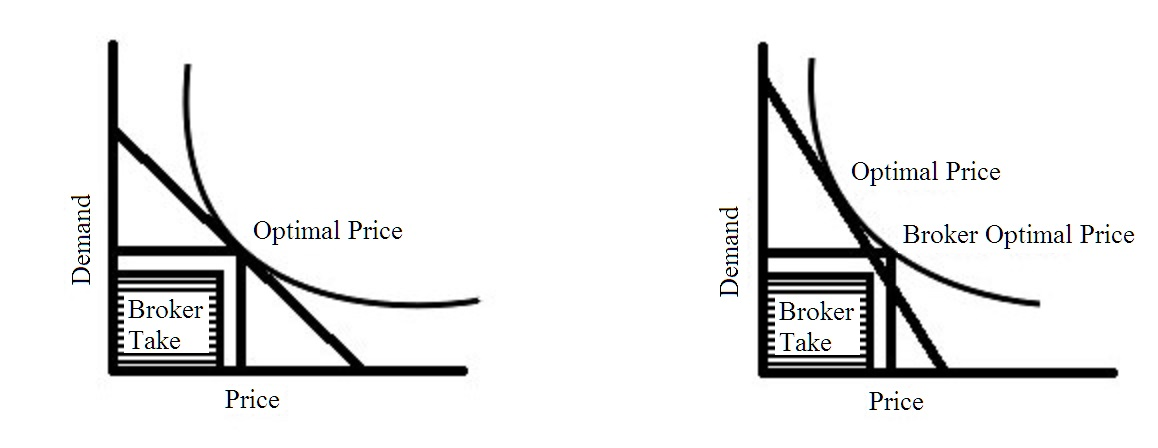
\includegraphics[scale=.3]{IMG_20151201_112640407.jpg}
	\caption{An optimal Pricing Choice for the Broker}
	\label{fig:demc}
\end{figure}

\section{Conclusion}
We have presented measures that enable us to effectively capture the nuances of the ticketing industry and enable a more effective analysis of the factors affecting ticket prices. As the prevalence of dynamic pricing increases in the industry, more sophisticated techniques will be needed to ensure the accuracy of prices leading to revenue maximization. A key element of the process is the ability to measure the phenomenon to be able to use past data and perform a causal analysis. 

We believe current regression techniques can be used with greater effect in understanding the nature of ticket sales over the lifecycle of an event using the measures defined. With sufficient data on events and ticket sales, logistic regression techniques can be used to identify the types of events that admit greater incidence of early vs late ticket sales, and influence the characteristics for improved revenues or better fan experience. The airline industry has similarly conditioned the consumers into buying the tickets as early as possible with effective price management.

Similarly, the price measures can be effectively used in analysis of price changes on a day-to-day basis. These analyses will become indispensable as the need to change ticket prices on a more frequent basis arises, and an unbiased estimation of the various factors affecting ticket price can only be achieved by adjusting for varying ticket quality on sale on a daily basis. Additionally, the event level price indices can be used for more effective cross-section analysis of event prices.

\bibliographystyle{agsm}
\bibliography{ref}
\end{document}

